\documentclass[9pt]{beamer}

\usepackage{ucs}
\usepackage[utf8x]{inputenc}
% \usepackage{beamerthemeplain}

\usepackage{amsmath}
\usepackage{amsfonts}
\usepackage{amssymb}
\usepackage[english]{babel}
\usepackage{fontenc}
% \usepackage{verbatim}
\usepackage{graphics}
 
\usepackage{textcomp}
\usepackage[absolute,overlay]{textpos}

\usepackage{wasysym}

\usepackage{slashed}
\usepackage{array}

\usetheme{CNRScolors}

\newcommand{\afac}[1]{\noindent \textcolor{red}{{\small \sc #1}}}

\usepackage{xspace}
%units
\usepackage[squaren,Gray,mediumqspace,thinspace,textstyle]{SIunits}

\usepackage[permil]{overpic}

\usepackage{textcomp}
\usepackage[absolute,overlay]{textpos}

\newcommand{\egamma}{E_{\gamma}}
\newcommand{\unitMass}{\giga\electronvolt/c^2}
\newcommand{\unitMom}{\giga\electronvolt/c}
\newcommand{\GeV}{\giga\electronvolt}
\newcommand{\TeV}{\tera\electronvolt}
\newcommand{\fb}{\femto\barn}
\newcommand{\pb}{\pico\barn}
\newcommand{\invmub}{\micro\reciprocal\barn}
\newcommand{\invpb}{\pico\reciprocal\barn}
\newcommand{\invfb}{\femto\reciprocal\barn}
\newcommand{\invnb}{\nano\reciprocal\barn}
\newcommand{\lumi}{\ensuremath{\mathcal{L}}}
\newcommand{\lumiunit}{\centi\meter\rpsquared\usk\reciprocal\second}
\newcommand{\pomeron}{\mathbb{P}}
\newcommand{\xp}{x_\pomeron}
\newcommand{\dkap}{\ensuremath{\Delta\kappa^{\gamma}}}
\newcommand{\kap}{\ensuremath{\kappa^{\gamma}}}
\newcommand{\lam}{\ensuremath{\lambda^{\gamma}}}
\newcommand{\aOw}{\ensuremath{a_0^W}}
\newcommand{\aOz}{\ensuremath{a_0^Z}}
\newcommand{\aCw}{\ensuremath{a_C^W}}
\newcommand{\aCz}{\ensuremath{a_C^Z}}
\newcommand{\aOwL}{\ensuremath{a_0^W/\Lambda^2}}
\newcommand{\aOzL}{\ensuremath{a_0^Z/\Lambda^2}}
\newcommand{\aCwL}{\ensuremath{a_C^W/\Lambda^2}}
\newcommand{\aCzL}{\ensuremath{a_C^Z/\Lambda^2}}
% \newcommand{\Lcutoff}{\ensuremath{\Lambda_{\text{cutoff}}}}
\newcommand{\Lcutoff}{\ensuremath{\Lambda}}
\newcommand{\wwgamma}{WW\gamma}
\newcommand{\missET}{\ensuremath{\not\!\!E_T}}
\newcommand{\etmiss}{\ensuremath{\not\!\!E_T}}
\newcommand{\WWgg}{\ensuremath{WW\gamma\gamma}}
\newcommand{\ggWW}{\ensuremath{WW\gamma\gamma}}
\newcommand{\dd}{\mathop{}\mathopen{}\text{d}}

\newcommand{\gpU}[1]{\ensuremath{\text{U}({#1})}}
\newcommand{\gpSU}[1]{\ensuremath{\text{SU}({#1})}}
\newcommand{\gpO}[1]{\ensuremath{\text{O}({#1})}}
\newcommand{\gpSO}[1]{\ensuremath{\text{SO}({#1})}}

\newcommand{\DO}{D\O{}\xspace}

\newcommand{\ith}{\textsuperscript{th}}
\newcommand{\st}{\textsuperscript{st}}
\newcommand{\nd}{\textsuperscript{nd}}
\newcommand{\rd}{\textsuperscript{rd}}

% \myfig[width=3cm]{label}{images/Chap1/myfig.pdf}{The capture of my figure.}
\newcommand{\myfig}[4][width=0.7\textwidth]{%
\begin{center}
 \begin{figure}
  \includegraphics[#1]{#3}
  
 \caption{\label{#2} #4}
 \end{figure}
\end{center}
}

\newcommand\FrameText[1]{%
  \begin{textblock*}{\paperwidth}(0pt,33pt)
    \raggedleft \small #1\hspace{.5em}
  \end{textblock*}}

\newcommand{\myincgr}[4]{
     \begin{overpic}[#1]{#2}
     \put(#3){#4}
     \end{overpic}}
\newcommand{\myincgrduo}[6]{
     \begin{overpic}[#1]{#2}
     \put(#3){#4}
     \put(#5){#6}
     \end{overpic}}
{\newcommand{\cmsSymbolFace}{\text}
\newcommand{\PT}{\ensuremath{p_{\text{T}}}\xspace}
\newcommand{\pt}{\ensuremath{p_{\text{T}}}\xspace}
\newcommand{\cm}{\ensuremath{\,\text{cm}}\xspace}
\newcommand{\PGm}{\ensuremath{\mu}\xspace} % muon
% \newcommand{\GeV}{\ensuremath{{\,\text{Ge\hspace{-.08em}V}}}\xspace}
\newcommand{\GeVc}{\ensuremath{{\,\text{Ge\hspace{-.08em}V\hspace{-0.16em}/\hspace{-0.08em}}c}}\xspace}
\newcommand{\GeVcc}{\ensuremath{{\,\text{Ge\hspace{-.08em}V\hspace{-0.16em}/\hspace{-0.08em}}c}^2}\xspace}
\newcommand{\abs}[1]{\ensuremath{\lvert #1 \rvert}}

% frequently used expressions
\newcommand{\ee}{\ensuremath{e^+e^-}\xspace}
\newcommand{\mumu}{\ensuremath{\mu^+\mu^-}\xspace}
\newcommand{\Mmumu}{\ensuremath{m_{\mu\mu}}\xspace}
\newcommand{\mmumu}{\ensuremath{m_{\mu\mu}}\xspace}
\newcommand{\eexp}[1]{\ensuremath{{\text e}^{#1}}\xspace}

% \newcommand{\qqbar}{\ensuremath{{\cmsSymbolFace{q}\overline{\cmsSymbolFace{q}}}}\xspace}
\newcommand{\QQbar}{\ensuremath{{\cmsSymbolFace{Q}\overline{\cmsSymbolFace{Q}}}}\xspace}
\newcommand{\Jpsi}{\ensuremath{\cmsSymbolFace{J}\hspace{-.08em}/\hspace{-.14em}\psi}\xspace}
\newcommand{\JPsi}{\ensuremath{\cmsSymbolFace{J}\hspace{-.08em}/\hspace{-.14em}\psi}\xspace}
\newcommand{\psiP}{\ensuremath{\psi\text{(2S)}}\xspace}
\newcommand{\B}{\ensuremath{\cmsSymbolFace{B}}\xspace}
\newcommand{\D}{\ensuremath{\cmsSymbolFace{D}}\xspace}

% \newcommand{\doubleRatio}{\ensuremath{\left.\left[N_{\psiP}/N_{\Jpsi}\right]_{\PbPb}\middle/\left[N_{\psiP}/N_{\Jpsi}\right]_{\pp}\right.\xspace}}
\newcommand{\doubleRatio}{\ensuremath{\left.(N_{\psiP}/N_{\Jpsi})_{\PbPb}/(N_{\psiP}/N_{\Jpsi})_{\pp}\right.\xspace}}

\newcommand{\PgU}{\ensuremath{\Upsilon}\xspace}
\newcommand{\PgUa}{\ensuremath{\Upsilon\text{(1S)}}\xspace}
\newcommand{\PgUb}{\ensuremath{\Upsilon\text{(2S)}}\xspace}
\newcommand{\PgUc}{\ensuremath{\Upsilon\text{(3S)}}\xspace}
\newcommand{\PgUbc}{\ensuremath{\Upsilon\text{(2S+3S)}}\xspace}
\newcommand{\PgUabc}{\ensuremath{\Upsilon\text{(1S,2S,3S)}}\xspace}
\newcommand{\PgUn}{\ensuremath{\Upsilon\text{(nS)}}\xspace}

\newcommand{\W}{\ensuremath{\cmsSymbolFace{W}}\xspace}
%\newcommand{\Z}{\ensuremath{\cmsSymbolFace{Z}}\xspace}
\newcommand{\ttbar}{\ensuremath{\cmsSymbolFace{t}\bar{\cmsSymbolFace{t}}}\xspace}

\newcommand{\dndy}{\ensuremath{dN/dy}\xspace}
\newcommand{\dnchdy}{\ensuremath{dN_{\text{ch}}/dy}\xspace}
\newcommand{\dndeta}{\ensuremath{dN/d\eta}\xspace}
\newcommand{\dnchdeta}{\ensuremath{dN_{\text{ch}}/d\eta}\xspace}
\newcommand{\dndpt}{\ensuremath{dN/d\pt}\xspace}
\newcommand{\dnchdpt}{\ensuremath{dN_{\text{ch}}/d\pt}\xspace}
\newcommand{\deta}{\ensuremath{\Delta\eta}\xspace}
\newcommand{\dphi}{\ensuremath{\Delta\phi}\xspace}
\newcommand{\phistar}{\ensuremath{\phi^*}\xspace}

\newcommand {\npart}  {\ensuremath{N_{\text{part}}}\xspace}
\newcommand {\ncoll}  {\ensuremath{N_{\text{coll}}}\xspace}

\newcommand{\AAA}{\ensuremath{\text{AA}}\xspace}
\newcommand{\raa}{\ensuremath{R_{\AAA}}\xspace}
\newcommand{\rpa}{\ensuremath{R_{\text{pA}}}\xspace}
\newcommand{\taa}{\ensuremath{T_{\AAA}}\xspace}
\newcommand{\rfb}{\ensuremath{R_\text{FB}}\xspace}

% references to equations, figures or tables
\newcommand{\eq}[1]{Eq.~\eqref{#1}\xspace}
\newcommand{\fig}[1]{Fig.~\ref{#1}\xspace}
\newcommand{\tab}[1]{Table~\ref{#1}\xspace}

% collision types
\newcommand{\pp}{{\ensuremath{\text{pp}}}\xspace}
\newcommand{\ppbar}{\ensuremath{\text{p}\overline{\text{p}}}\xspace}
\newcommand{\pPb}{\ensuremath{\text{p}\text{Pb}}\xspace}
\newcommand{\ppb}{\ensuremath{\text{p}\text{Pb}}\xspace}
\newcommand{\PbPb}{\ensuremath{\text{PbPb}}\xspace}
\newcommand{\pbpb}{\ensuremath{\text{PbPb}}\xspace}
\newcommand{\AuAu}{\ensuremath{\text{AuAu}}\xspace}

% center of mass energy
\newcommand{\sqrts}{\ensuremath{\sqrt{s}}\xspace}
\newcommand{\sqrtsnn}{\ensuremath{\sqrt{s_{_{\text{NN}}}}}\xspace}

%units
\newcommand{\mbinv} {\mbox{\ensuremath{\,\text{mb}^\text{$-$1}}}\xspace}
%\newcommand{\mubinv} {\mbox{\ensuremath{\,\mu\text{b}^\text{$-$1}}}\xspace}

% program name
\providecommand{\CASCADE} {{\textsc{cascade}}\xspace}
\providecommand{\HYDJET} {{\textsc{hydjet}}\xspace}


% ljpsi
\newcommand{\Lxy}{\ensuremath{L_{xy}}\xspace}
\newcommand{\Lxyz}{\ensuremath{L_{xyz}}\xspace}
% \newcommand{\ctau}{\ensuremath{c\tau^{2D}}\xspace}
% \newcommand{\ctauxyz}{\ensuremath{c\tau^{3D}}\xspace}
\newcommand{\ctau}{\ensuremath{\ell_{\Jpsi}^{2D}}\xspace}
\newcommand{\ctauxyz}{\ensuremath{\ell_{\Jpsi}^{3D}}\xspace}

% pPb 
\newcommand{\etalab}{\ensuremath{\eta_\text{lab}}\xspace}

\graphicspath{ {../figures/}{./} }

\setbeamertemplate{navigation symbols}{}

 \newcolumntype{x}[1]{%
>{\centering\hspace{0pt}}p{#1}}%
\newcommand{\tn}{\tabularnewline}

\date[Stat2]{Sept. 27, 2018}
\title{Methods of statistical analysis and simulation}
\subtitle{Cours 2}
\author[E. Chapon]{Émilien Chapon}
% \institute[(CERN)]{CERN}
% \logo{\includegraphics[height=0.6cm]{../../CMS-Color-Label.pdf}\hspace{1.05\textwidth}\includegraphics[height=0.6cm]
% {../../LogoBadge.pdf} }

\begin{document}

{
\setbeamertemplate{footline}{}
\setbeamertemplate{headline}{}
% \logo{\includegraphics[height=1.2cm]{../../CMS-Color-Label.pdf}
% \hspace{0.94\textwidth}\includegraphics[height=1.2cm]{../../LogoBadge.pdf}}

\begin{frame}
 \maketitle
 
%  \setcounter{framenumber}{0}
\end{frame}
}


% CONTENU
% point estimation... cf cours ED, compléter avec le F. James

\begin{frame}
 \frametitle{Outline}
 
 \tableofcontents
\end{frame}

\section{Information}

\begin{frame}
 \frametitle{The likelihood function}
 
 We discuss a random variable $X$, with pdf $f(X|\theta)$, where $\theta$ is a real parameter (or a set of $k$ real parameters).
 The set of allowed values of $X$ is denoted $\Omega_\theta$.
 
 We consider $N$ independent observations of $X$: $X_1,\dots,X_N$. The joint pdf is, by independence,
 
 $$P(\vec{X}|\theta) = P(X1,\dots,X_N)|\theta) = \prod_{i=1}^N f(X_i|\theta)$$
 
 \begin{block}{Likelihood function}
  The likelihood function is a function of $\theta$, given the observed data $X^0$:
  
  $$\mathcal{L}(\theta) = P(X^0|\theta)$$
 \end{block}

  
\end{frame}

\begin{frame}
 \frametitle{Notes on the likelihood function}
 
 \begin{itemize}
  \item It is tempting to consider the area under $\mathcal{L}$, but $\mathcal{L}(\theta)$ is not a probability distribution function in $\theta$: \alert{the area under $\mathcal{L}$ is meaningless}.
  \item We will see that likelihood ratios are often used.
 \end{itemize}


\end{frame}

\begin{frame}
 \frametitle{Likelihood function: example}
 
 \begin{itemize}
  \item Poisson probability $P(n|\mu) = \mu^n \frac{e^{-\mu}}{n!}$
  \item Suppose $n=3$ is observed. We get the likelihood function:
  $$\mathcal{L}(\mu) = \mu^3 \frac{e^{-\mu}}{3!}$$
 \end{itemize}
 
 \begin{center}
  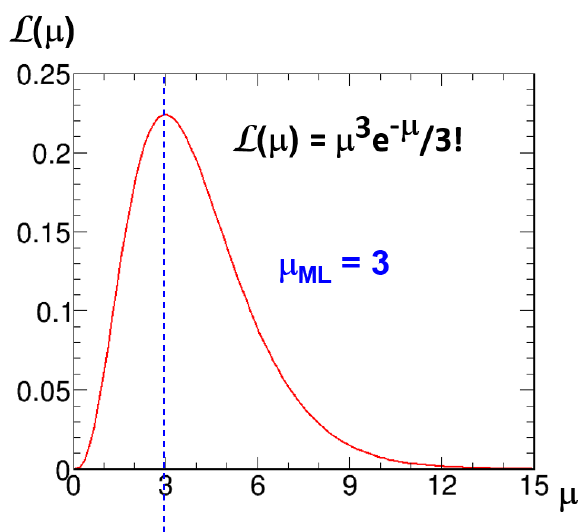
\includegraphics[width=0.6\textwidth]{likelihood_Poisson.png}
 \end{center}


\end{frame}


\begin{frame}
 \frametitle{Statistic}
 
 \begin{block}{Definition}
  Suppose a new random variable: $T = T(X_1,\dots,X_N)$. Any such function $T$ is called a \textbf{statistic}.
 \end{block}
 
 Example: sample mean $\bar{X}$.
 
 \vspace{10pt}
 
 NB: careful not to confuse this \textbf{statistic} with \textbf{statistics} (the field of mathematics we are discussing) or \textbf{statistics} (physicist's jargon as a substitute for
 ``data'' or ``amount of data''. Better avoid the latter usage when writing papers!

\end{frame}

\begin{frame}
 \frametitle{Information of R.A. Fisher}
 
 \begin{block}{Definition}
 If $\Omega_\theta$ is independent of $\theta$, and if $\mathcal{L}(X|\theta)$ is regular enough to allow the operators $\partial^2/\partial\theta^2$ and $\int \dd X$ to comute, then
  \begin{eqnarray}
   I_X(\theta) & = & E \left[ \left( \frac{\partial \ln \mathcal{L}(X|\theta)}{\partial \theta} \right)^2 \right] \nonumber \\
   & = & \int_{\Omega_\theta} \left( \frac{\partial \ln \mathcal{L}(X|\theta)}{\partial \theta} \right)^2 \mathcal{L}(X|\theta) \dd X
  \end{eqnarray}

 \end{block}
 
 NB: this is an additive property (the information of $N$ observations is $N$ times the information of 1 observation).

\end{frame}


\begin{frame}
 \frametitle{Sufficient statistics}
 
 \begin{block}{Definition}
  A statistic is said to be \textbf{sufficient} if $f(\vec{X}|T)$ is independent of $\theta$.
 \end{block}
 
 Properties:
 
 \begin{itemize}
  \item If $T$ is a sufficient statistic for $\theta$, then any strictly monotonic function of $T$ is also a sufficient statistic for $\theta$.
  \item $T(\vec{X})$ is a sufficient statistic for $\theta$ iff the likelihood factorises as
  $$\mathcal{L}(\vec{X}|\theta) = g(T,\theta) h(\vec{X}),$$
  where:
  \begin{enumerate}
   \item $h(\vec{X})$ does not depend on $\theta$
   \item $g(T,\theta) \propto A(T|\theta)$, the conditional pdf for $T$ given $\theta$.
  \end{enumerate}
 \end{itemize}


\end{frame}

\begin{frame}
 \frametitle{Darmois theorem}
 
 This theorem proves that only a very restricted class of probability density functions admits a number of sufficient statistics independent of the number of observations.
 
 \begin{itemize}
  \item Whatever $\Omega_\theta$, if there exists a number $N>1$ such that the set $X1,\dots,X_N$ admits a sufficient statistic for $\theta$, then the pdf is of the ``exponential form''
  $$f(X|\theta) = \exp [ \alpha(X)a(\theta) + \beta(X) + c(\theta)]$$
  \item Inversely, $(X1,\dots,X_N)$ admits a sufficient statistic for all $N>1$ (but only if $\Omega_\theta$ does not depend on $\theta$), if $f(X|\theta)$ has the exponential form,
  and if the mapping $(X_1,\dots,X_N) \Rightarrow (R,X_2,\dots,X_N)$, with
  $$R = \sum_{i=1}^N \alpha(X_i),$$
  is one-to-one and continuously differentiable for all $X$. $R$ is sufficient for $\theta$, as well as any monotonic function of $R$.
 \end{itemize}

\end{frame}



\section{Point estimation}

\begin{frame}
 \frametitle{Outline}
 
 \tableofcontents[current]
\end{frame}


\begin{frame}
 \frametitle{Parameter estimation}
 
 Let $X$ be a random variable of pdf $f(x;\theta_0)$, with $\theta_0$ unknown. We draw $N$ independent trials of $X$, $\{x_1,\dots,x_N\}$.
 
 
 An \textbf{estimator} is a statistic $t_N(x_1,\dots,x_N)$ that can be used to estimate $\theta_0$. It can have the following properties:
 
 \begin{description}
  \item[unbiased]: if $\langle t_N \rangle = \theta_0$ (otherwise the bias is $\langle t_N \rangle - \theta_0 = b_N$)
  \item[convergent] or consistent: e.g. consistency in probability, $\forall \epsilon>0, \forall \eta>0, \exists N_0 / \forall N>N_0, P(|t_N - \theta_0|>\epsilon)<\eta$
  \begin{itemize}
   \item NB: The law of large numbers is equivalent to the statement that the sample mean is a consistent estimator of the parent mean.
  \end{itemize}
  \item[efficient]: if $t_N$ is unbiased and that its variance $V(t_N) \xrightarrow[N\to\infty]{} \text{minimum variance}$ (this property can be only asymptotic)
  \item[optimal]: if $t_N$ is unbiased and reaches the minimum variance bound
  \item[robust]: if it does not depend on a hypothesis on the pdf
 \end{description}

\end{frame}

\begin{frame}
 \frametitle{Illustration}
 
 pdfs for $t_N$ in different cases
 
 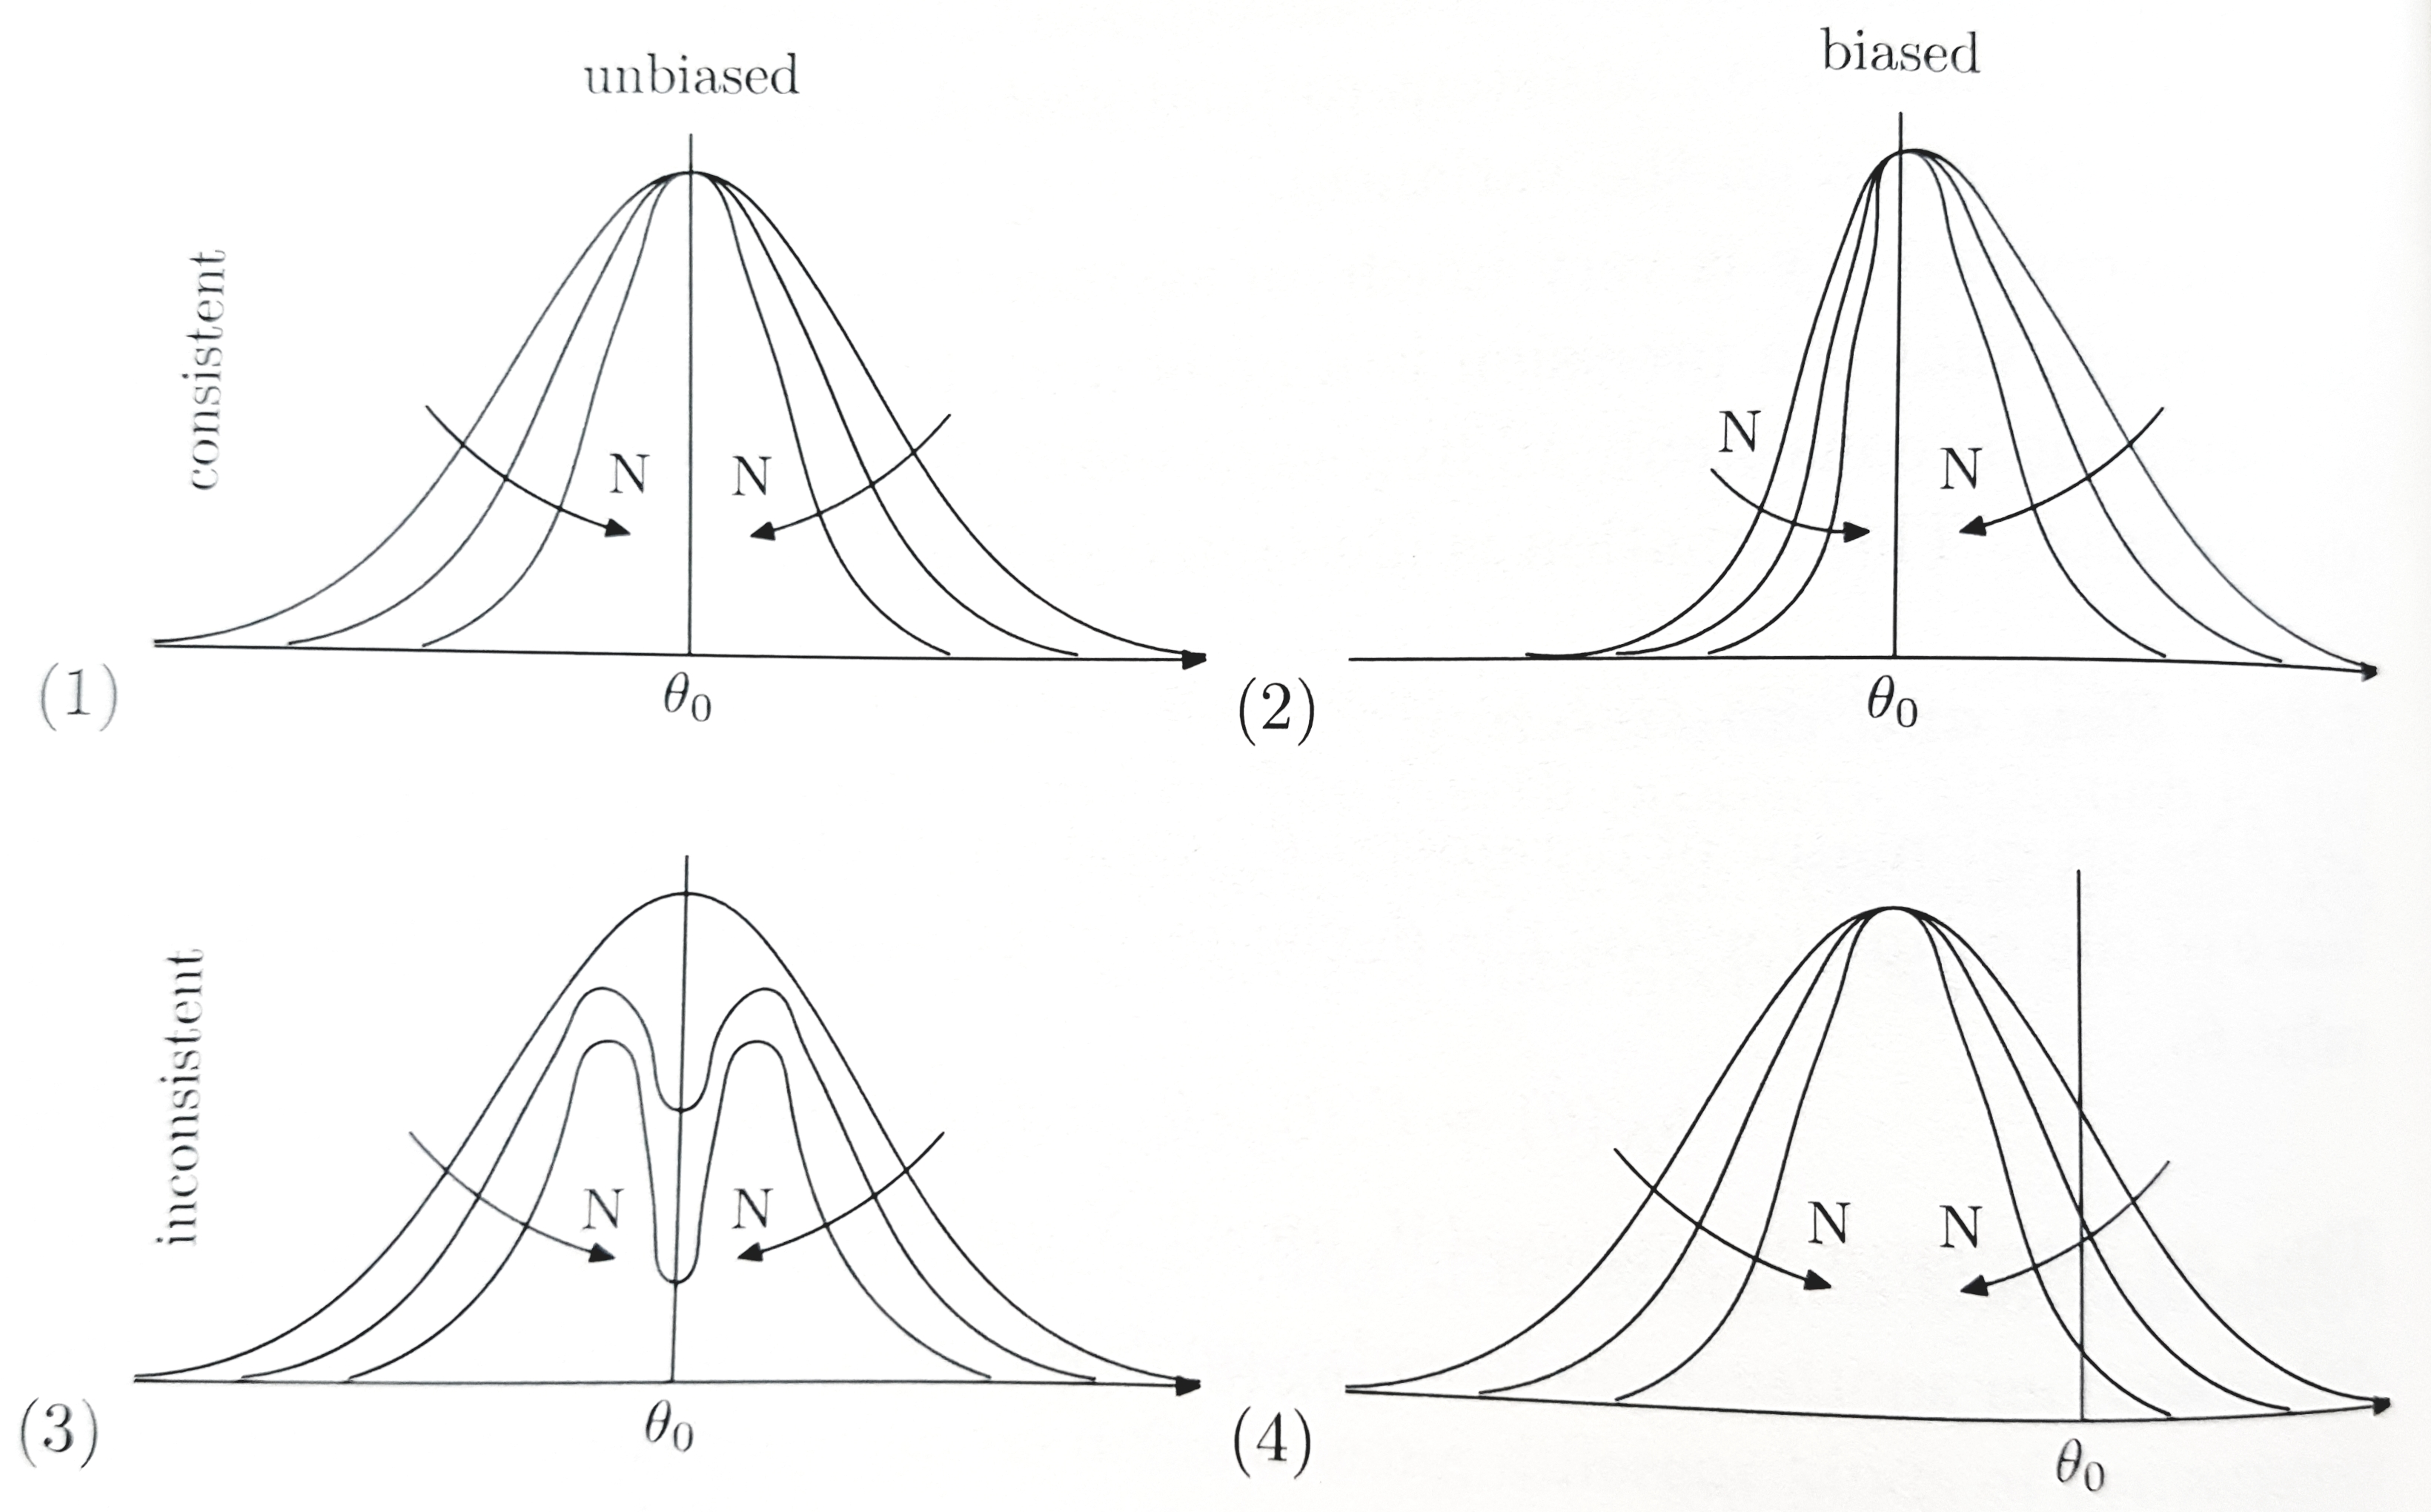
\includegraphics[width=\textwidth]{estimators.jpg}
\end{frame}


\begin{frame}
 \frametitle{Minimum variance: Cramér-Rao inequality}
 
 Let $\vec{X}$ be observations from a distribution with pdf $f(\vec{X}|\theta)$, the likelihood is $\mathcal{L}_{\vec{X}} = L(\vec{X}|\theta)$.
 
 \begin{block}{Cramér-Rao inequality}
 If the range of $\vec{X}$ does not depend on $\theta$, and if $\mathcal{L}_{\vec{X}}$ is sufficiently regular that differentiation with respect fo $\theta$ and integration over 
 $\theta$ commute, then:
 
  $$V(\hat{\theta}) \geq \frac{[1+(\dd b / \dd \theta)]^2}{I_{\hat{\theta}}} 
  \geq \frac{[1+(\dd b / \dd \theta)]^2}{I_{\vec{X}}} 
  = \frac{\left( \frac{\dd \tau(\theta)}{\dd \theta} \right)^2}{E\left[ \left( \frac{\partial \ln \mathcal{L}_{\vec{X}}}{\partial \theta} \right)^2 \right]}$$
  
  where $I_{\vec{X}}$ is the Fisher information, $I_{\vec{X}}(\theta) = E\left[ \left( \frac{\partial \ln \mathcal{L}(\vec{X}|\theta)}{\partial \theta} \right)^2 \right]$, and 
  $\tau(\theta) \equiv E(\hat{\theta}) = \theta + b(\theta)$
 \end{block}

\end{frame}

\begin{frame}
 \frametitle{Efficiency and minimum variance}
 
 \begin{block}{First part of the inequality: minimum variance}
  $V(\hat{\theta}) = \frac{[1+(\dd b / \dd \theta)]^2}{I_{\hat{\theta}}} $ iff the sampling distribution of $\hat{\theta}$ is of the exponential form:
  
  $$\mathcal{L}_{\hat{\theta}} = \exp [a(\theta)\hat{\theta} + \beta(\hat{\theta}) + c(\theta)]$$
 \end{block}
 
 \begin{block}{Second part of the inequality: minimum bound variance (efficient estimator)}
  $V(\hat{\theta}) = \frac{[1+(\dd b / \dd \theta)]^2}{I_{\vec{X}}} $ iff $ I_{\hat{\theta}} = I_{\vec{X}} $, ie iff $\hat{\theta}$ is a sufficient statistic for $\theta$, ie
  iff $f(\vec{X}|\theta)$ is of the exponential form (Darmois' theorem).
 \end{block}


\end{frame}


\begin{frame}
 \frametitle{Usual methods of constructing consistent estimators}
 
 We can use the law of large numbers:
 
 $$\frac{1}{N} \sum_{i=1}^N a(X_i) \xrightarrow[N\to\infty]{} E[a(X)] = \int a(X)f(X,\theta_0)\dd X$$
 
 We will see:
 
 \begin{itemize}
  \item the moments method
  \item the maximum likelihood method
 \end{itemize}

 
\end{frame}


\begin{frame}
 \frametitle{The moments method}
 
 Let $a(X)$ such that $E[a(X)] = \int a(X) f(X;\theta) \dd X = h(\theta)$ where $h$ is known. 
 
 If $h$ is invertible, we can find the true value of $\theta$: 
 $\theta_0 = h^{-1}(E[a]) = h^{-1}\left(\int a(X) f(X;\theta) \dd X\right)$
 
 The estimator is then:
 
 $$\hat{\theta} = h^{-1} \left( N^{-1} \sum_{i=1}^N a(x_i) \right)$$
 
 NB: $\hat{\theta}$ does not directly depend on $f$, only on the $x_i$.
\end{frame}

\begin{frame}
 \frametitle{The moments method: application}
 
 \begin{block}{1D case ($\theta \in \mathbb{R}$)}
  We take simply $a(X) = X$. Then $h(\theta_0) = \bar{X} = \mu$: it is the sample mean.
 \end{block}
 
 \begin{block}{ND case: $\vec{\theta} = (\theta_1,\dots,\theta_K)$}
  We take $a_j(X) = X^j$. Then $h_j(\vec{\theta}) = \mu_j(\vec{\theta})$: $j$-ith moment of $f(X;\vec{\theta})$
 \end{block}


\end{frame}

\begin{frame}
 \frametitle{The maximum likelihood method (ML)}
 
 In general the logarithm of $\mathcal{L}$ is used: $\ln \mathcal{L}\left(\vec{X};\theta\right) = \sum_{i=1}^N \ln f(X_i;\theta)$
 
 \begin{block}{Maximum likelihood estimator}
  $$\left. \frac{\partial (\ln \mathcal{L} \left(\vec{X};\theta\right)}{\partial \theta}\right|_{\hat{\theta}_\text{ML}} = \left.\frac{\partial}{\partial \theta} \left(  \sum_{i=1}^N \ln f(X_i;\theta) \right)\right|_{\hat{\theta}_\text{ML}} = 0$$
  
  $\hat{\theta}_\text{ML}$ is the maximum likelihood estimator of $\theta$.
 \end{block}

 Note: numerical methods are often designed to look for a minimum rather than a maximum. $-2 \ln \mathcal{L}$ is more commonly used.
\end{frame}

\begin{frame}
 \frametitle{The maximum likelihood estimator (MLE)}
 
 This estimator is 
 \begin{itemize}
  \item asymptotically efficient
  \item biased (except when the likelihood is of the exponential form)
  \item non optimal (except when the likelihood is of the exponential form)
  \item convergent
  \item invariant: the ML estimate $\hat{\tau}$ of a function $\tau(\theta)$ is $\hat{\tau} = \tau(\hat{\theta})$
  \begin{itemize}
   \item However other properties of the MLE (e.g. the bias) are not invariant under change of parameter.
  \end{itemize}

 \end{itemize}

\end{frame}

\begin{frame}
 \frametitle{Variance of the MLE}
 
 $$V(\hat{\theta}_{ML}) \xrightarrow[N\to\infty]{} \frac{1}{N} \left[ \left.-E\left(\frac{\partial^2\ln f(x;\theta)}{\partial \theta^2}\right)\right|_{\theta=\theta_0} \right]^{-1} \approx \frac{1}{D_2(\theta=\hat{\theta}_{ML})}$$
 
\end{frame}

\begin{frame}
 \frametitle{(Academic) example of a poor MLE}
 
 One observed $N$ events $X_i$ from a uniform distribution in $[0,\theta]$, where $\theta$ is \textbf{unknown}. 
 
 \begin{itemize}
  \item The likelihood function is $\mathcal{L} = \prod_{i=1}^N \theta^{-1} = \theta^{-N}$ and the MLE is $\hat{\theta} = \max\{X_i\}$.
  \item The MLE is biased (always to small by definition)... intuitively $\hat{\theta}_{CS} = \max\{X_i\} + \max\{X_i\}/N$ is a better estimate.
 \end{itemize}
\end{frame}

\begin{frame}
 \frametitle{(Academic) example of a poor MLE}
 
 \begin{center}
  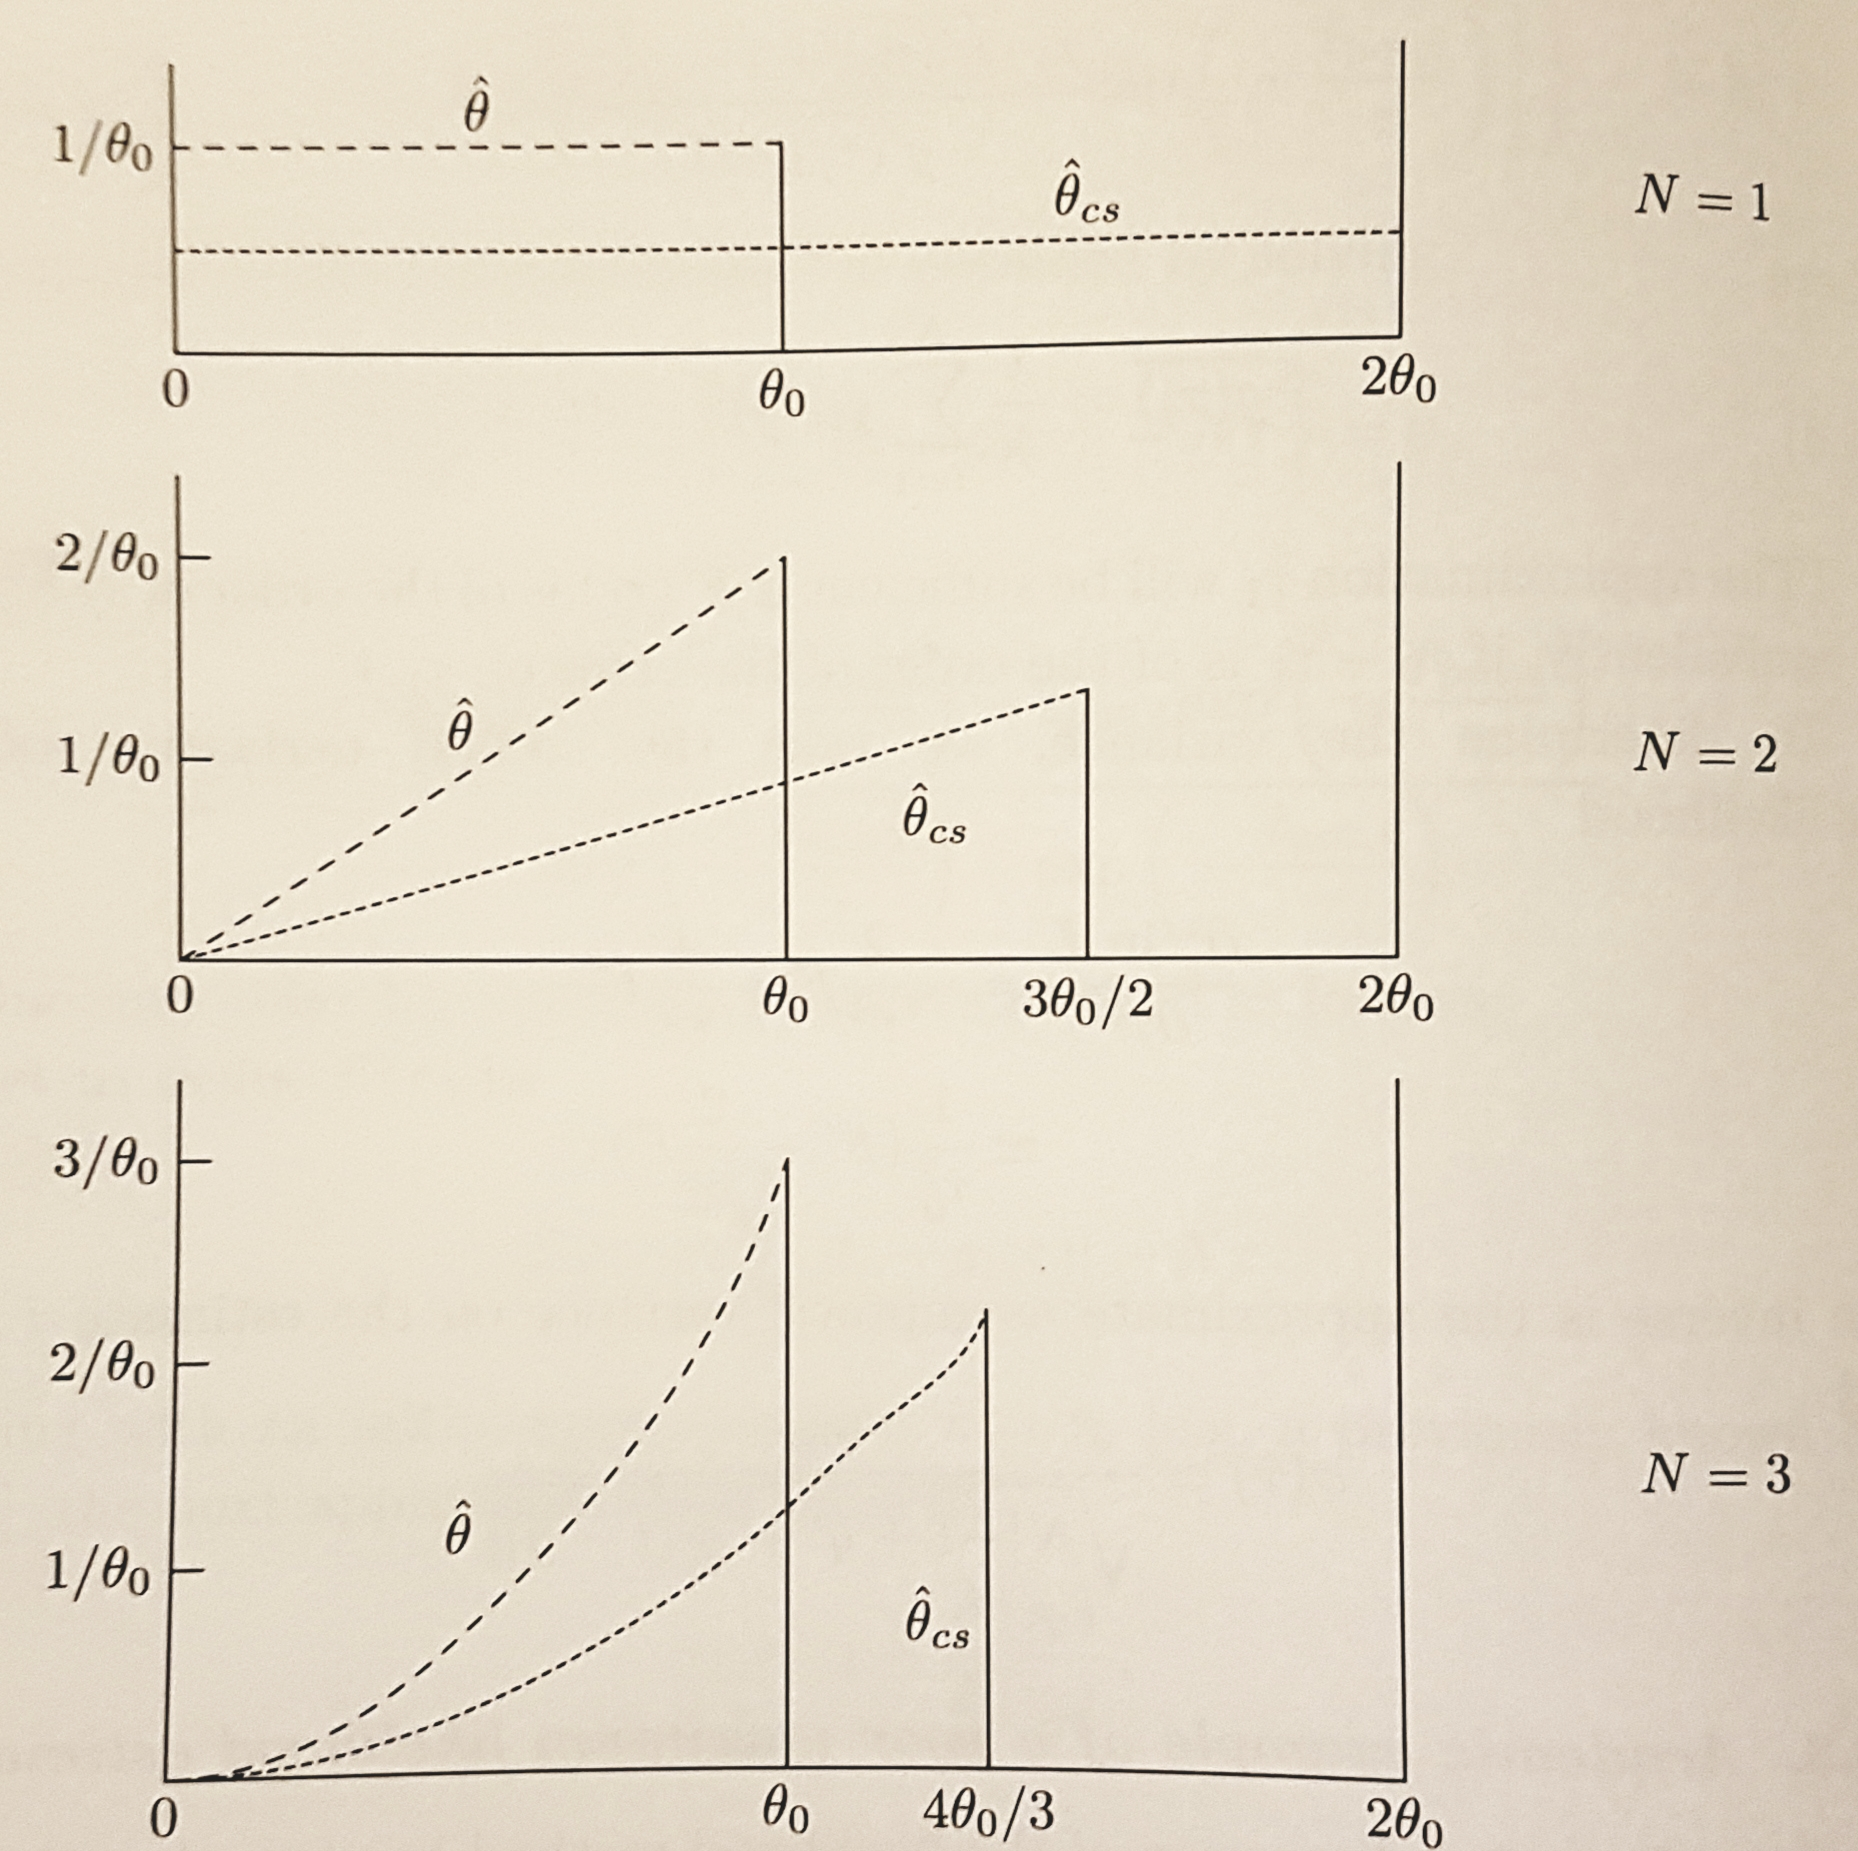
\includegraphics[width=0.7\textwidth]{academic_MLE.jpg}
 \end{center}

\end{frame}



\section{Least squares method}

\begin{frame}
 \frametitle{Outline}
 
 \tableofcontents[current]
\end{frame}

\begin{frame}
 \frametitle{Least squares method (aka $\chi^2$ estimator)}
 
 We consider $N$ observations $\vec{x}$
 
 $E(x_i;\vec{\theta})$ and $V_{ij}(\vec{\theta})$ ($i,j = 1\dots N$) are \textbf{known functions} of $\vec{\theta}$
 
 \begin{block}{Least squares estimator}
 The estimator is the value $\vec{\theta}$ such that $Q$ is minimum:
 
  $$Q = \left[ \vec{X} - E(\vec{X};\vec{\theta}\right]^\intercal V^{-1} (\vec{\theta}) \left[ \vec{X} - E(\vec{X};\vec{\theta}) \right]$$
  
  $$Q = \sum_{i=1}^N \sum_{j=1}^N \left[ X_i - E(X_i;\vec{\theta})\right] V^{-1}_{ij} \left[ X_j - E(X_j;\vec{\theta})\right]$$
 \end{block}
 
 This estimator is:
 
 \begin{itemize}
  \item consistent
  \item (generally) biased
  \item non-optimal
 \end{itemize}


\end{frame}

\begin{frame}
 \frametitle{Gaussian case}
 
 In the Gaussian case, the least squares and maximum likelihood methods coincide. Assuming $N$ independent measurements $y_i$ at known points $x_i$, Gaussian distributed with mean
 $\mu(x_i;\theta)$ and known variance $\sigma_i^2$:
 
 $$\chi^2(\theta) = -2\ln\mathcal{L}(\theta) + \text{constant} = \sum_{i=1}^N \frac{\left(X_i - \mu(\theta)\right)^2}{\sigma_i^2}$$
\end{frame}


\begin{frame}
 \frametitle{$\chi^2$ estimator: uncorrelated case}
 
 Uncorrelated case: $V_{ij} = 0 $ for $i \neq j$
 
 $$Q = \sum_{i=1}^N \frac{\left(x_i - E(x_i; \vec{\theta})\right)^2}{\sigma_i^2(\vec{\theta})}$$
\end{frame}

\begin{frame}
 \frametitle{Variance of the $\chi^2$ estimator}
 
 If $\theta \in \mathbb{R}$:
 
 $$V(\hat{\theta}_{LS}) \xrightarrow[N\to\infty]{} 2\left(\left.\frac{\partial^2 Q}{\partial\theta^2}\right|_{\theta=\theta_0}\right)^{-1} \approx \frac{2}{D_2(\theta=\hat{\theta}_{LS})}$$
\end{frame}


\begin{frame}
 \frametitle{Specific cases of the $\chi^2$ estimator}
 
 \begin{block}{Linear case}
  If $\sigma_i$ are independent of $\theta$, and $E(x_k;\theta)$ linear function of $\theta$: $Q$ is optimal and convergent
 \end{block}
 
 \begin{block}{Gaussian case}
  If the $x_i$ follow a normal law $G(X_i;\mu_i,\sigma_i)$: $Q$ follows a $\chi^2$ law, $\chi^2(Q;N)$:
  
  $$\chi^2(\vec{\theta}) = \sum_{i=1}^N \frac{\left( X_i - \mu_i (\vec{\theta})\right)^2}{\sigma_i^2 (\vec{\theta})}$$
  
  If in addition the model is linear ($\sigma_i$ independent of $\theta$): $\chi^2_\text{min} = \chi^2 (\chi^2_\text{min};N-r)$ (with $r$ the dimension of $\vec{\theta}$), and $\vec{\theta}_{LS}$ follows a normal law of dimesion $r$ with $\langle \hat{\theta}_{LS}\rangle = \vec{\theta}_0$, $V = 2 D_2^{-1}$
  
 \end{block}


\end{frame}

\section{Parameter estimation with histograms}

\begin{frame}
 \frametitle{Outline}
 
 \tableofcontents[current]
\end{frame}

\begin{frame}
 \frametitle{}
 
 Let's assume an histogram with $N$ uncorrelated bins (the total number of events is not fixed): $d_i$ events in bin $i$, with $i = 1 \dots N$. The $d_i$ follow Poisson laws: $E(d_i;\theta) = f_i(\theta)$,
 $\sigma^2(d_i;\theta) = f_i(\theta)$.
 
 \begin{block}{Minimum $\chi^2$ method}
 Expected uncertainties: 
 
  $$Q_P = \sum_{i=1}^N = \frac{\left(d_i - f_i\right)^2}{f_i^2}$$
 \end{block}
 
 \begin{block}{Modified minimum $\chi^2$ method}
 Observed uncertainties:
 
  $$Q_N = \sum_{i=1}^N = \frac{\left(d_i - f_i\right)^2}{d_i^2}$$
 \end{block}
 
 \begin{block}{Binned likelihood}
  $$\ln \lambda = \sum_{i=1}^N d_i \ln f_i$$
 \end{block}



\end{frame}

\begin{frame}
 \frametitle{}
 
 The three methods are asymptotically equivalent. The binned likelihood method converges faster (and the modified $\chi^2$ is the slowest), and is less sensitive to empty bins. 
\end{frame}

\section{Some basic estimators}


\begin{frame}
 \frametitle{Outline}
 
 \tableofcontents[current]
\end{frame}

\begin{frame}
 \frametitle{Sample mean}
 
 $$\bar{X} = \sum_{i=1}^N \frac{x_i}{N} = \bar{mu}$$
 
 This estimator is unbiased, thanks to the central limit theorem.
 
 Its variance is:
 
 $$V(\hat{\mu}) = \frac{\sigma^2}{N},\qquad\text{i.e.}\quad \sigma(\hat{\mu}) = \frac{\mu}{\sqrt{N}}$$
 
 The sample mean is an efficient estimator of the mean of a Gaussian, but not in the general case.
\end{frame}

\begin{frame}
 \frametitle{Variance estimator: known mean}
 
 $$\hat{V}_\mu = \frac{1}{N} \sum_{i=1}^N (x_i-\mu)^2$$
 
 This estimator is consistent and unbiased: $\langle \hat{V}_\mu \rangle = \frac{N\langle (x-\mu)^2 \rangle}{N} = V$
\end{frame}

\begin{frame}
 \frametitle{Variance estimator: unknown mean}
 
 Using $\hat{\mu} = \bar{X}$
 
 $$\hat{V}_b = \frac{1}{N} \sum_{i=1}^N (x_i-\bar{X})^2 = \frac{1}{N} \sum_{i=1}^N (x_i^2 - \bar{X}^2)$$
 
 \begin{eqnarray}
  \langle \hat{V}_b \rangle & = & \frac{N \langle X^2 - \bar{X}^2 \rangle}{N} = \langle X^2 \rangle - \langle \bar{X} \rangle^2 \nonumber \\
  & = & \langle X^2 \rangle - \langle X \rangle^2 - \left( \langle \bar{X}^2 \rangle - \langle \bar{X} \rangle ^2 \right) \nonumber \\
  & = & V(X) - V(\bar{X}) \nonumber \\
  & = & V(X) - \frac{V(X)}{N} \nonumber \\
  & = & \left( 1 - \frac{1}{N} \right) V(X)\quad \neq V(X) \nonumber
 \end{eqnarray}
 
 This estimator is biased! $\rightarrow$ Bessel correction

\end{frame}

\begin{frame}
 \frametitle{Variance estimator: unknown mean}

 \begin{block}{}
  $$\hat{V} = \frac{1}{N-1} \sum_{i=1}^N (x_i - \bar{X})^2$$
 \end{block}
 
 $$V(\hat{V}) = \frac{2V}{N}$$

\end{frame}

\section{Point estimation in practice}

\begin{frame}
 \frametitle{Outline}
 
 \tableofcontents[current]
\end{frame}

\begin{frame}
 \frametitle{Choice of estimator}
 How to choose an estimator? It should have the following properties:
 
 \begin{itemize}
  \item Consistency and unbiasedness
  \item Minimum loss of information
  \item Minimum variance (efficient estimator)
  \item Robustness
  \item Simplicity (e.g. if possible normally distributed, etc.)
  \item Minimum computer time
  \item Minimum loss of physicist's time
 \end{itemize}

\end{frame}

\subsection{More realistic cases}

% cf Fred James + PDG stat review

\begin{frame}
 \frametitle{Extended likelihood}
\end{frame}

\begin{frame}
 \frametitle{Nuisance parameters}
\end{frame}


\section{Data combination}

\begin{frame}
 \frametitle{Outline}
 
 \tableofcontents[current]
\end{frame}


\begin{frame}
 \frametitle{Combination of data}
 
 BLUE, etc
\end{frame}


\end{document}

